%=========================================================================
% (c) 2014, 2015 Josef Lusticky

\section{IP stack}\label{sec:linux-ip}
The Linux IPv4 stack, or simply the IP stack, claims to be the most RFC-compliant network stack available~\cite{linux-foundation-toe}.
The functions found in the IPv4 stack are responsible for handling IPv4 packets only.
IPv6 packets are handled by the IPv6 stack, which is different,
however, most of the principles of IPv4 processing, apply to IPv6 processing as well~\cite{linux-kernel-networking}.

Figure~\ref{fig:linux-ingress-packet} shows the core functions of the IP stack for ingress packet processing in the Linux kernel.
For the sake of simplicity, the figure shows no IPsec, Fragmentation or IP-Options processing.
The NF\_IP\_* items represent places where the Netfilter hooks can be applied.
Netfilter is an internal kernel framework for packet filtering,
network address translation, port translation, and more~\cite{netfilter}.
Netfilter can be manipulated from user-space using the {\it{iptables}} utility.

\begin{figure}
	\centering
	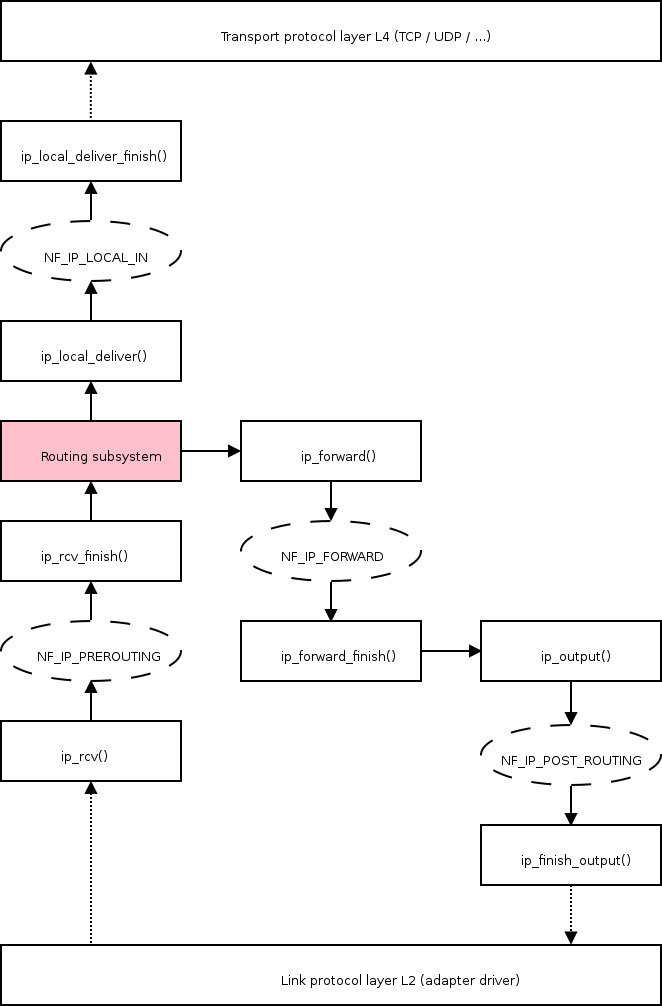
\includegraphics[width=12cm,keepaspectratio]{fig/kernel-layer3-flow.png}
	\caption{Ingress packet processing in the IPv4 stack}
	\label{fig:linux-ingress-packet}
	\bigskip
\end{figure}

The {\it{ip\_rcv()}} function performs mostly sanity checks -
IP version, IP checksum and header length are checked~\cite{kernel-source}.
If the received packet passes all the checks, it proceeds to the NF\_INET\_PRE\_ROUTING hook callback,
if such callback is registered.
If it was not discarded by the netfilter hook,
the {\it{skb}} associated with the packet is passed to the {\it{ip\_rcv\_finish()}} function,
where a lookup in the routing subsystem is performed.
The routing subsystem mainly assigns the {\it{skb$\rightarrow$\_skb\_refdst}} and it is further discussed in section~\ref{sec:linux-routing}.

Depending on the routing decision, the packet is either dropped with no further processing
or passed to the {\it{ip\_local\_deliver()}} function in case
the local host is the destination, or to the {\it{ip\_forward()}} function in case it needs to be forwarded~\cite{linux-kernel-networking}.
Packets to be delivered on the local host are passed to a higher-layer protocol handler (e.g. TCP)
for further processing.

Packets that are going to be forwarded are passed to the {\it{ip\_forward()}} function.
This function checks and decrements the value of the Time To Live (ttl) field in the IPv4 header.
If it reaches 0, the packet is discarded and an ICMPv4 message with "TTL Count Exceeded" code is sent back~\cite{linux-kernel-networking}.
Moreover, each time a packet is being
forwarded and the TTL is decremented by 1,
the checksum of the IPv4 header must be recalculated,
as its value depends on the IPv4 header, and the TTL is one of the IPv4 header members.
These tasks are done by the {\it{ip\_forward()}} function~\cite{linux-kernel-networking}.
The output processing function for the {\it{skb}} is further set to {\it{ip\_output()}}.
The packet is then passed to the {\it{ip\_forward\_finish()}} function,
which updates forwarding statistics and invokes the output processing function~\cite{linux-kernel-networking}.

The {\it{ip\_output()}} function updates transmission statistics and
assigns the output device to the {\it{skb$\rightarrow$dev}} member.
The packet is then passed to the {\it{ip\_finish\_output()}} function,
which must fragment the packet in case it is larger than the MTU of the {\it{skb$\rightarrow$dev}} device.
The function further takes care of neighboring using Address Resolution Protocol (ARP)~\cite{kernel-source}.
The neighboring subsystem is outside the scope of this thesis,
but in case the link-layer address of the destination is not known,
the packet transmission can be significantly delayed.
